
\documentclass[10pt,landscape]{scrartcl}

\usepackage[english]{babel}
% \usepackage[ngerman]{babel}
\usepackage[utf8]{inputenc}

\usepackage{lmodern}

\usepackage{ifthen}

\usepackage{graphicx}
% \usepackage{pstricks}
% \usepackage{relsize}
% \usepackage[decimalsymbol=comma,exponent-product = \cdot, per=frac]{siunitx}
% \sisetup{range-phrase=\,bis\,}

\usepackage{xargs}
\usepackage{calc}
\usepackage{amsmath}
\usepackage{amsfonts}
\usepackage{mathtools}
\usepackage{amssymb}

\usepackage{cancel}
\usepackage{trfsigns}
\usepackage{array}
\usepackage{enumerate}
\usepackage{enumitem}

\usepackage{caption}
\usepackage{subcaption}

\usepackage{multicol}

\usepackage{pdflscape}
\usepackage[table]{xcolor}

\usepackage{float}

%%%%%%%%%%%%%%%%%%%%%%%%%%%%%%%%%%%%%%%%%%%%%%%%%%%%%%%%%%%%%%%%%%%%%%%%%%%%%%%%
\newboolean{WITHPSTRICKS}
\setboolean{WITHPSTRICKS}{false}


\newcommand{\PROFESSOR}{Prof.\ Dr.\ Thomas Carraro}
\newcommand{\ASSISTANT}{\setlength{\tabcolsep}{0pt}\begin{tabular}{l} Dr. Ulrike Kochan-Eilers\end{tabular}}

\newcommand{\Jahr}{2025}
% \newcommand{\Trimester}{HT}
\newcommand{\Trimester}{WT}
\newcommand{\Kurs}{Mathematik II/B (WI/ET)}
\newcommand{\TYPE}{Aufgabenblatt}
\newcommand{\BLATT}{1}
\newcommand{\TOPIC}{Funktionsgraphen, Grenzwerte, Folgen, Differenzieren}

%%%%%%%%%%%%%%%%%%%%%%%%%%%%%%%%%%%%%%%%%%%%%%%%%%%%%%%%%%%%%%%%%%%%%%%%%%%%%%%%
\newboolean{mitLoes}
\setboolean{mitLoes}{false}
%\setboolean{mitLoes}{true}

%%%%%%%%%%%%%%%%%%%%%%%%%%%%%%%%%%%%%%%%%%%%%%%%%%%%%%%%%%%%%%%%%%%%%%%%%%%%%%%%


%\setboolean{WITHPSTRICKS}{false}
%\setboolean{WITHPSTRICKS}{true}


\usepackage{tikz}
\usetikzlibrary{arrows,automata,backgrounds,calendar,decorations.pathmorphing,fadings,shadings,calc,intersections}
\usetikzlibrary{decorations.pathreplacing}
\usetikzlibrary{decorations.shapes}
\usetikzlibrary{decorations.footprints}
\usetikzlibrary{decorations.text}
\usetikzlibrary{positioning}
\usetikzlibrary{through}
\usepackage[utf8]{inputenc}


\ifthenelse{\boolean{WITHPSTRICKS}}{%
\usepackage{auto-pst-pdf}
\usepackage{pstricks,pst-plot,pst-text}
}{}

\usepackage{pgfplots}

%%%%%%%%%%%%%%%%%%%%%%%%%%%%%%%%%%%%%%%%%%%%%%%%%%%%%%%%%%%%%%%%%%%%%%%%%%%%%%%%
\usepackage{mbdefAufgaben}

%%%%%%%%%%%%%%%%%%%%%%%%%%%%%%%%%%%%%%%%%%%%%%%%%%%%%%%%%%%%%%%%%%%%%%%%%%%%%%%%
\newboolean{mitErg}
%\setboolean{mitErg}{false}

%%%%%%%%%%%%%%%%%%%%%%%%%%%%%%%%%%%%%%%%%%%%%%%%%%%%%%%%%%%%%%%%%%%%%%%%%%%%%%%%
\newcounter{Aufg}
\setcounter{Aufg}{0}
\newcounter{Blatt}
\setcounter{Blatt}{1}

%%%%%%%%%%%%%%%%%%%%%%%%%%%%%%%%%%%%%%%%%%%%%%%%%%%%%%%%%%%%%%%%%%%%%%%%%%%%%%%%
%\usepackage{KopfEnglish}

% Seitenraender
%\textwidth = 285mm
%\textheight = 180mm
%\leftmargin 5mm
%\oddsidemargin = -20mm
%\evensidemargin = -20mm
%\topmargin = -25mm
%\parindent 0cm
%\columnsep 2cm

% % % Aufgabenstellung
% % % Schwierungkeitsgrad mit "e" , "f" oder "v" angeben
% % % "e" Einführung   
% % % "f" Festigung
% % % "v" Vertiefung  

\newcommand{\Aufgabe}[3][]{
\stepcounter{Aufg}
\subsubsection*{Aufgabe 
\arabic{Aufg}\ifthenelse{\equal{#1}{e}}{}{\ifthenelse{\equal{#1}{f}}{
$\!\!{}^\star$}{\ifthenelse{\equal{#1}{v}}{$^{\star\star}$}{}}}{: #2}}
{#3}
}
% % % Ergebnisse jeweils am Ende des Aufgabenblattes Anzeigen
\newcommand{\Ergebnisse}{}
\makeatletter
\newcommand{\Ergebnis}[1]{
	\g@addto@macro{\Ergebnisse}{#1}
}
\makeatother
\makeatletter
\newcommand{\ErgebnisC}[2]{
\@ifundefined{c@#1}
{\newcounter{#1}}
{}
\setcounter{#1}{\theAufg}

\ifthenelse{\boolean{mitErg}}{	\g@addto@macro{\Ergebnisse}{\subsubsection*{Ergebnisse zu Aufgabe \arabic{#1}:}
}%
	\g@addto@macro{\Ergebnisse}{#2}}{}
}
\makeatother


% % % Lösungen
\newcommand{\Loesung}[1]{
	\ifthenelse{\boolean{mitLoes}}
	{\subsubsection*{Lösung \arabic{Aufg}:}
		#1}
	{}
}
% % % % % % % % % % % % % % % % % % % % % % % % % % % % % % % % % % % % % % % % % % % % % % % % % % % % % %
% % % % % % % % % % % % % % % % % % % % % % % % % % % % % % % % % % % % % % % % % % % % % % % % % % % % % %
% % % % % % % % % % % % % % % % % % % % % % % % % % % % % % % % % % % % % % % % % % % % % % % % % % % % % %
\begin{document}
%\begin{twocolumn}
% % % % % % % % % % % % % % % % % % % % % % % % % % %

%%%%%%%%%%%%%%%%%%%%%%%%%%%%%%%%%%%%%%%%%%%%%%%%%%%%%%%%%%%%%%%%%%%%%%%%%%%%%%%%
% Set the TITLE of the sheet here:
%\uebheader{\Kurs}{\arabic{Blatt}}{\Trimester\,\Jahr}{\TOPIC}
%\uebheader{\Kurs}{\arabic{Blatt}}{\Trimester\,\Jahr}{\TOPIC}
%\uebheader{\Kurs}{\arabic{Blatt}}{\Trimester\,\Jahr}{\TOPIC}
%\ruleBig

\setboolean{mitErg}{false}
 \setboolean{mitErg}{true}


%%%%%%%%%%%%%%%%%%%%%%%%%%%%%%%%%%%%%%%%%%%%%%%%%%%%%%%%%%%%%%%%%%%%%%%%%%%%%%%%
% Set the INTRODUCTION section of the sheet here:
% \input{introduction.tex}

\textbf{Einführende Bemerkungen}

\begin{itemize}
\item Vermeiden Sie die Verwendung von Taschenrechnern oder Online-Ressourcen.
% \item Die mit einem Stern *) markierten (Teil-)Aufgaben entfallen in diesem Trimester. Stattdessen werden einzelne Online-Aufgaben im ILIAS-Kurs kenntlich gemacht, zu denen Sie dort Ihre L\"osungswege zur Korrektur hochladen k\"onnen. 
% \item Die mit zwei Sternen  **) markierten (Teil-)Aufgaben richten sich an Studierende, die die \"ubrigen Aufgaben bereits gel\"ost haben und die Inhalte weiter vertiefen m\"ochten. 
\end{itemize}

\ruleBig

%Mathe II Blatt 1
\Aufgabe[e]{~} {
%Plot each of the following functions in a coordinate system individually,
%label the data axes and highlight significant values.
Stellen Sie jede der folgenden Funktionen einzeln in einem Koordinatensystem dar, beschriften Sie die Datenachsen und heben Sie signifikante Werte hervor (z.B. Maxima/Minima, Nullstellen, usw.).

\begin{abc}
\item $p_1(x)=2x-1$

\item $p_2(x)=(x-2)^2-1$

\item $p_3(x)=x^3$

\item $p_4(x)=-x^3$


\item $f_1(x)=\sin(x+\frac{\pi}{2})$

\item $f_2(x)=-\cos(x)$

\item $f_3(x)=\sin(x)$

\item $f_4(x)=\tan x$


\item $g_1(x)=\sqrt{x}$

\item $g_2(x)=\displaystyle \frac{1}{x}$

\item $g_3(x)=\displaystyle \frac{1}{x^2}$


\item $h_1(x)=\ln x$

\item $h_2(x)=\ln x +1$

\item $h_3(x)=\ln(x+1)$


\item $i_1(x) = \exp(x)$

\item $i_2(x) = \exp(-x)$

\end{abc}

}


\Loesung{

\textbf{a)} $p_1(x)=2x-1$

\begin{minipage}{\linewidth}
\centering

\begin{tikzpicture}
\begin{axis}[
axis lines=middle,
clip=false,
xmin=-pi,
xmax=3*pi,
ymin=-5.9,
ymax=5.9,
xlabel=$x$,
ylabel=$f(x)$,
xticklabel style={black}
]

\addplot[domain=-1.7:2.9,samples=200,blue]{2*x-1}
node[right,pos=.9,font=\footnotesize]{$p_1(x)$};

\end{axis}
\end{tikzpicture}

\end{minipage}


\bigskip
\textbf{b)} $p_2(x)=(x-2)^2-1$

\begin{minipage}{\linewidth}
\centering

\begin{tikzpicture}
\begin{axis}[
axis lines=middle,
clip=false,
xmin=-pi,
xmax=3*pi,
ymin=-5.9,
ymax=5.9,
xlabel=$x$,
%ylabel=$y$,
xticklabel style={black}
]

\addplot[domain=-0.5:4.5,samples=200,blue]{(x-2)^2-1}
node[right,pos=.9,font=\footnotesize]{$p_2(x)$};

\end{axis}
\end{tikzpicture}

\end{minipage}

\newpage
\bigskip
\textbf{c)}  $p_3(x)=x^3$

\bigskip
\textbf{d)}  $p_4(x)=-x^3$


\begin{minipage}{\linewidth}
\centering

\begin{tikzpicture}
\begin{axis}[
axis lines=middle,
clip=false,
xmin=-pi,
xmax=3*pi,
ymin=-5.9,
ymax=5.9,
xlabel=$x$,
%ylabel=$y$,
xticklabel style={black}
]
\addplot[domain=-1.75:1.75,samples=200,blue]{x^3}
node[right,pos=.9,font=\footnotesize]{$x^3$};

\addplot[domain=-1.75:1.75,samples=200,red,densely dashed]{-x^3}
node[right,pos=.9,font=\footnotesize]{$-x^3$};

\end{axis}
\end{tikzpicture}

\end{minipage}

%\bigskip
\textbf{e)} $f_1(x)=\sin(x+\frac{\pi}{2}) = \cos(x)$

\bigskip
\textbf{f)} $f_2(x)=-\cos(x)$

\begin{minipage}{\linewidth}
\centering

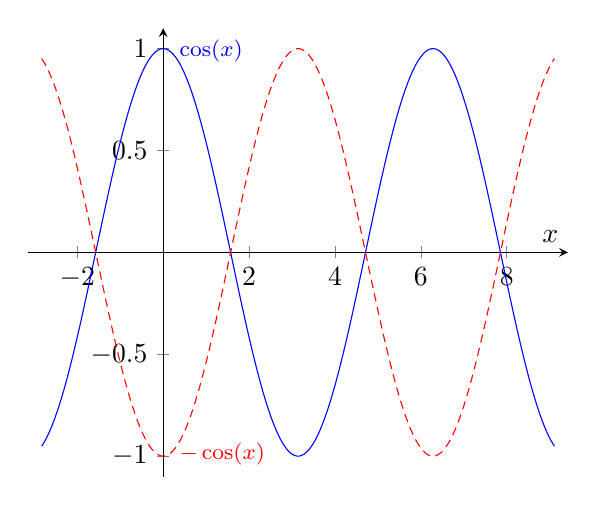
\begin{tikzpicture}
\begin{axis}[
axis lines=middle,
clip=false,
xmin=-pi,
xmax=3*pi,
ymin=-1.1,
ymax=1.1,
xlabel=$x$,
%ylabel=$y$,
xticklabel style={black}
]

\addplot[domain=-.9*pi:2.9*pi,samples=200,blue]{cos(deg(x))}
node[right,pos=.25,font=\footnotesize]{$\cos(x)$};

\addplot[domain=-.9*pi:2.9*pi,samples=200,red,densely dashed]{-cos(deg(x))}
node[right,pos=.25,font=\footnotesize]{$-\cos(x)$};

\end{axis}
\end{tikzpicture}

\end{minipage}

\newpage
\bigskip
\textbf{g)} $f_3(x)=\sin(x)$

\begin{minipage}{\linewidth}
\centering

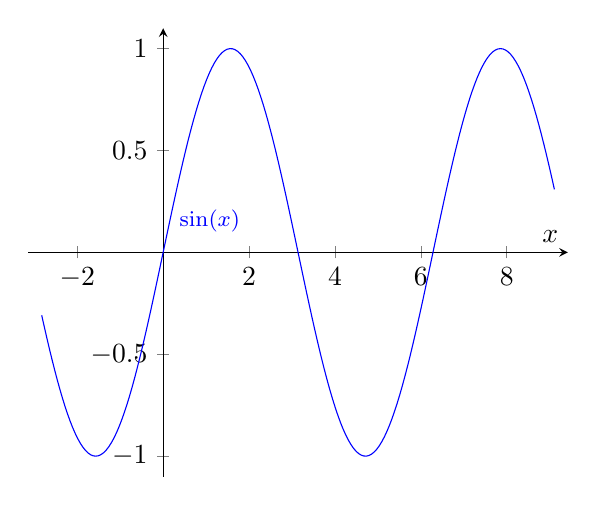
\begin{tikzpicture}
\begin{axis}[
axis lines=middle,
clip=false,
xmin=-pi,
xmax=3*pi,
ymin=-1.1,
ymax=1.1,
xlabel=$x$,
%ylabel=$y$,
xticklabel style={black}
]

\addplot[domain=-.9*pi:2.9*pi,samples=200,blue]{sin(deg(x))}
node[right,pos=.25,font=\footnotesize]{$\sin(x)$};


\end{axis}
\end{tikzpicture}

\end{minipage}

\bigskip
\textbf{h)} $f_4(x)= \tan x$

\begin{minipage}{\linewidth}
\centering

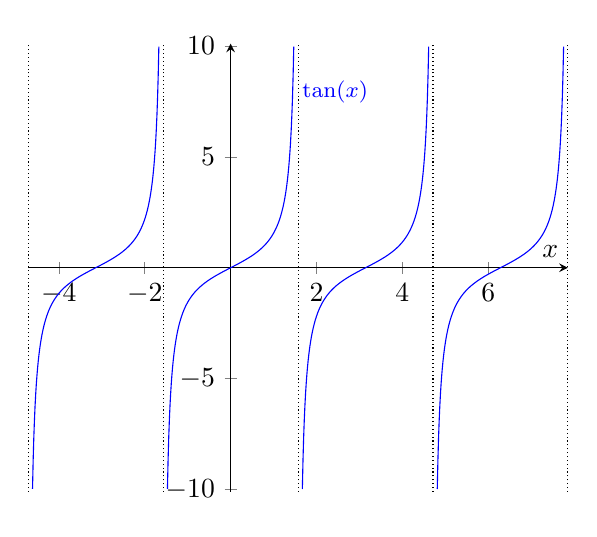
\begin{tikzpicture}
\begin{axis}[
axis lines=middle,
clip=false,
xmin=-1.5*pi,
xmax=2.5*pi,
ymin=-10.1,
ymax=10.1,
xlabel=$x$,
%ylabel=$y$,
xticklabel style={black}
]

\addplot[mark=none,black,densely dotted] coordinates {(-pi/2-pi, -10.1) (-pi/2-pi, 10.1)};

\addplot[domain=-pi/2+.1-pi:pi/2-.1-pi,samples=200,blue]{tan( deg(x) )};

\addplot[mark=none,black,densely dotted] coordinates {(-pi/2, -10.1) (-pi/2, 10.1)};

\addplot[domain=-pi/2+.1:pi/2-.1,samples=200,blue]{tan( deg(x) )}
node[right,pos=0.9,font=\footnotesize]{$\tan(x)$};

\addplot[mark=none,black,densely dotted] coordinates {(-pi/2+pi, -10.1) (-pi/2+pi, 10.1)};

\addplot[domain=-pi/2+.1+pi:pi/2-.1+pi,samples=200,blue]{tan( deg(x) )};

\addplot[mark=none,black,densely dotted] coordinates {(-pi/2+2*pi, -10.1) (-pi/2+2*pi, 10.1)};

\addplot[domain=-pi/2+.1+2*pi:pi/2-.1+2*pi,samples=200,blue]{tan( deg(x) )};

\addplot[mark=none,black,densely dotted] coordinates {(-pi/2+3*pi, -10.1) (-pi/2+3*pi, 10.1)};

\end{axis}
\end{tikzpicture}

\end{minipage}


\newpage
\bigskip
\textbf{i)} $g_1(x)=\sqrt{x}$

\begin{minipage}{\linewidth}
\centering

\begin{tikzpicture}
\begin{axis}[
axis lines=middle,
clip=false,
xmin=-1.1,
xmax=3.9,
ymin=-1.1,
ymax=3.9,
xlabel=$x$,
ylabel=$f(x)$,
xticklabel style={black}
]

\addplot[domain=0:3.7,samples=200,blue]{sqrt(x)}
node[right,pos=.1,font=\footnotesize]{$\sqrt{x}$};

\end{axis}
\end{tikzpicture}

\end{minipage}


\bigskip
\textbf{j)} $g_2(x)=\displaystyle \frac{1}{x}$

\bigskip
\textbf{k)} $g_3(x)=\displaystyle \frac{1}{x^2}$

\begin{minipage}{\linewidth}
\centering

\begin{tikzpicture}
\begin{axis}[
axis lines=middle,
clip=false,
xmin=-4.9,
xmax=4.9,
ymin=-3.9,
ymax=3.9,
xlabel=$x$,
%ylabel=$f(x)$,
xticklabel style={black}
]

\addplot[domain=-4.7:-0.3,samples=200,blue]{1/x}
node[left,pos=.7,font=\footnotesize]{$\displaystyle \frac{1}{x}$};

\addplot[domain=0.3:4.7,samples=200,blue]{1/x}
node[left,pos=.3,font=\footnotesize]{$\displaystyle \frac{1}{x}$};


\addplot[domain=-4.7:-0.54,samples=200,red,densely dashed]{1/x^2}
node[left,pos=.7,font=\footnotesize]{$\displaystyle \frac{1}{x^2}$};

\addplot[domain=0.54:4.7,samples=200,red,densely dashed]{1/x^2};

\end{axis}
\end{tikzpicture}

\end{minipage}


\newpage
\bigskip
\textbf{l)} $h_1(x)=\ln x$

\begin{minipage}{\linewidth}
\centering

\begin{tikzpicture}
\begin{axis}[
axis lines=middle,
clip=false,
xmin=-1.1,
xmax=3.9,
ymin=-3.9,
ymax=3.9,
xlabel=$x$,
ylabel=$f(x)$,
xticklabel style={black}
]

\addplot[domain=0.025:3.7,samples=200,blue]{ln(x)}
node[right,pos=.1,font=\footnotesize]{$\ln(x)$};

\end{axis}
\end{tikzpicture}

\end{minipage}


\bigskip
\textbf{m)} $h_2(x)=\ln x +1$

\begin{minipage}{\linewidth}
\centering

\begin{tikzpicture}
\begin{axis}[
axis lines=middle,
clip=false,
xmin=-1.1,
xmax=3.9,
ymin=-3.9,
ymax=3.9,
xlabel=$x$,
ylabel=$f(x)$,
xticklabel style={black}
]

\addplot[domain=0.025:3.7,samples=200,blue]{ln(x)+1}
node[right,pos=.1,font=\footnotesize]{$\ln(x)+1$};

\addplot[domain=0:3.7,black,densely dotted]{1.0};

\end{axis}
\end{tikzpicture}

\end{minipage}


\newpage
\bigskip
\textbf{n)} $h_3(x)=\ln(x+1)$


\begin{minipage}{\linewidth}
\centering

\begin{tikzpicture}
\begin{axis}[
axis lines=middle,
clip=false,
xmin=-1.1,
xmax=3.9,
ymin=-3.9,
ymax=3.9,
xlabel=$x$,
ylabel=$f(x)$,
xticklabel style={black}
]

\addplot[domain=0.025-1:3.7,samples=200,blue]{ln(x+1)}
node[right,pos=.1,font=\footnotesize]{$\ln(x+1)$};

\addplot[mark=none,black,densely dotted] coordinates {(-1, -3.9) (-1, 0)};

\end{axis}
\end{tikzpicture}

\end{minipage}

\bigskip
\textbf{o)} $i_1(x)=\exp(x)$

\bigskip
\textbf{p)} $i_2(x)=\exp(-x)$

\begin{minipage}{\linewidth}
\centering

\begin{tikzpicture}
\begin{axis}[
axis lines=middle,
clip=false,
xmin=-3,
xmax=3,
ymin=-5,
ymax=20,
xlabel=$x$,
ylabel=$f(x)$,
xticklabel style={black}
]

\addplot[domain=-3:3,samples=200,blue]{exp(x)}
node[right,pos=.1,font=\footnotesize]{$\exp(x)$};

\addplot[domain=-3:3,samples=200,red,densely dashed]{exp(-x)}
node[right,pos=.1,font=\footnotesize]{$\exp(-x)$};

\end{axis}
\end{tikzpicture}

\end{minipage}
}

\ifthenelse{\boolean{mitLoes}}{\ruleBig \cleardoublepage}{}

\Aufgabe[e]{Grenzwertdefinition}{
Bestimmen Sie zu den unten angegebenen Folgen $(a_n)$ mit dem Grenzwert $a$ und den angegebenen
Werten f\"ur $k$ jeweils ein $N$ so, dass f\"ur alle $n\in \N$ mit $n>
N$ gilt 
$$|a_n-a|< 10^{-k}.$$
\begin{abc}
\item $a_n=\dfrac{1}{\sqrt n}$, $a=0$, $k=2$
\item $a_n=\dfrac{3n+1}{ n+1}$, $a=3$, $k=4$
\item $a_n=\dfrac{(-1)^n}{n!}+1$, $a=1$, $k=3$
\end{abc}
}

\Loesung{
\begin{abc}
\item Es soll gelten $|a_n-a|=\frac 1{\sqrt n}\overset !<10^{-2}$. Dies l\"asst sich umstellen zu: 
$$n>\left(\frac 1{10^{-2}}\right)^2=10^4=10000=N.$$
\item Hier ergibt sich 
\begin{align*}
&&|a_n-a|&<10^{-4}\\
\Leftrightarrow&& 10^{-4}&>\left|\frac{3n+1}{n+1}-3\right|=\frac{|-2|}{n+1}\\
\Leftrightarrow&& \frac{n+1}2&>10^4\\
\Leftrightarrow&& n&> 20000-1=19999=N. 
\end{align*}
\item F\"ur diese Folge ist $|a_n-a|=\left|\frac{(-1)^n}{n!}\right|=\frac 1{n!}$ Mit $k=3$ soll also
gelten: 
$$\frac 1{n!}<10^{-3}\quad\Leftrightarrow\quad n!>1000.$$
Das ist beispielsweise erf\"ullt f\"ur $n>1000=N$. Ein kleinstm\"ogliches $N$ kann man durch die
Untersuchung von $n!$ ermitteln. Es ist $6!=720<1000$ und $7!=7\cdot 6!=5040>1000$. 
Die Bedingung ist also bereits f\"ur $n>6$ erf\"ullt. 
\end{abc}
}

\ErgebnisC{analysGrenWert004}
{
\textbf{a)} $N=10000$, \textbf{b)} $N=19999$, \textbf{c)} $N=6$ 
}

\ifthenelse{\boolean{mitLoes}}{\ruleBig \cleardoublepage}{}

\Aufgabe[e]{~} {
\begin{abc}
 \item Zeigen Sie anhand der Definition der Konvergenz, dass gilt
\[
\lim_{n\rightarrow \infty} \dfrac{2n^2+n-12}{n^2-8} = 2\,.
\]

\item Zeigen Sie: Konvergiert $\{a_{n}\}_{n\in\N}$ gegen $a$, so konvergiert 
auch $\{|a_{n}|\}_{n\in\N}$ gegen $|a|$.

\item Gilt die Umkehrung von b)? Begr\"unden Sie Ihre Aussage mit einem
  Beweis oder einem Gegenbeispiel.

\end{abc}



}


\Loesung{
\bigskip
\textbf{L\"osung}

\smallskip
\textbf{Zu a)} Die Aussage \glqq $a_n$ konvergiert gegen $a$\grqq\ bedeutet: F\"ur jedes 
$k\in \N > 0$ existiert ein $N=N(k)\in \R$, so dass f\"ur alle $n > N$ gilt, dass 
$|a_n-a| < 10^{-k}$. F\"ur $n\in \N$ gilt:
$$
a_n := \dfrac{2n^2+n-12}{n^2-8} = \dfrac{2(n^2-8)+(n+4)}{n^2-8} = 2 + 
\dfrac{n+4}{n^2-8}\,.
$$
Damit folgt
\begin{align*}
|a_n - 2| & =  \left|\dfrac{n+4}{n^2-8}\right| \stackrel{\mbox{f\"ur }n\geq 3}{=} 
\dfrac{n+4}{n^2-8} = \dfrac{n+4}{n^2-16+8}\\[3ex]  & \stackrel{\mbox{f\"ur }n\geq 5}{<}  
\dfrac{n+4}{n^2-16} = \dfrac{n+4}{(n+4)(n-4)} = \dfrac{1}{n-4} \,.
\end{align*}
Sei nun $k\in \N$ vorgegeben. Es gilt 
\[
\frac{1}{n-4} = 10^{-k} \qquad \Longleftrightarrow \qquad n = 10^k +4\,.
\]
Ist $N(k):=4+10^k$, dann gilt insbesondere f\"ur alle $n > N(k)$: 
\[
 |a_n-2|< 10^{-k}\,. 
\]
Damit ist ist Behauptung bewiesen. 


\bigskip
\textbf{Zu b)} Die Aussage \glqq $a_n$ konvergiert gegen $a$\grqq\ bedeutet: F\"ur jedes 
$k\in \N$ gibt es ein $N(k)\in \R$, so dass f\"ur alle $n > N$ gilt, dass $|a_n-a| < 
10^{-k}$. Wegen 
\[
||a_n|-|a|| \le |a_n-a|\,,
\]
gilt f\"ur jedes $k\in \N$, dass das dazugeh\"orige $N(k)$ und jedes $n > N$ auch 
\[
||a_n|-|a|| <  10^{-k}
\] 
erf\"ullt, d.h.\ $|a_n|$ konvergiert gegen $|a|$.


\bigskip
\textbf{Zu c)} Die Umkehrung gilt nicht, zum Beispiel gilt f\"ur $a_n=(-1)^n$ sicher 
$|a_n|=1\to 1$, aber $(-1)^n$ ist nicht konvergent.

}

\ErgebnisC{aufgabe2}
{
\textbf{c)} Betrachten Sie $a_n=(-1)^n$. 
}

\ifthenelse{\boolean{mitLoes}}{\ruleBig \cleardoublepage}{}

\Aufgabe[e]{Differenzieren (Schulstoff)}{
Bestimmen Sie jeweils die erste Ableitung der folgenden Funktionen:
\begin{align*}
f_1(t)&=-\frac{1}{2}t^2-2t+6                         \,,&\quad  &&                       
f_2(t)&= \sqrt[3]{t}+1                       \,,&\quad  &&                              
f_3(t)&= \sin(\frac{t}{4\pi})                                \,,&\quad \\
f_4(t)&=  e^{t^2}   \,,&\quad  &&
f_5(t)&=  (\ln(t)) ^2                      \,,&\quad  &&
f_6(t)&=   \ln(e^t)                                 \,,&\quad \\ 
f_7(t)&=  t^3 \ln(t)-\frac{1}{2}t^2             \,,&\quad  && 
f_8(t)&=  \ln(\sqrt{t})  \,,&\quad  && 
f_9(t)    &= \sin(t)\cdot t^2                       \,,&\quad  \\
f_{10}(t) &=  \frac{1}{2}(t^2-2)^2.    
\end{align*}                                             
}

\Loesung{
\begin{align*}
f_1'(t)  & =  -t-2 = -(t+2)\,,\\[1ex]
f_2'(t)  & = (t^{\frac{1}{3}}+1)' = \frac{1}{3}t^{-\frac{2}{3}}\,,\\[1ex]
f_3'(t)  & =  \frac{1}{4\pi} \cdot \cos(\frac{t}{4\pi})\,,\\[1ex]
f_4'(t)  & =  2te^{t^2}  \,,\\[1ex]
f_5'(t)  & = \frac{2 \ln(t)}{t} \,,\\[1ex]
f_6'(t)  & = (t)' =1 \,,\\[1ex]
f_7'(t)  & = 3t^2 \ln(t)+t^2-t = t^2 (3 \ln(t)+1)-t     \,,\\[1ex]
f_8'(t)  & =  \frac{1}{\sqrt{t}}\frac{1}{2\sqrt{t}} = \frac{1}{2t} \,,\\[1ex]
f_9   '(t) & = \cos(t)t^2+\sin(t)2t=t(2\sin(t)+t\cos(t)) \,,\\[1ex]
f_{10}   '(t)& = 2t(t^2-2). \\
\end{align*}
}

\ErgebnisC{AufganalysDiffeinfach}
{
\begin{align*}
f_1'(t) =&     -(t+2)                      ,\,&\quad&& 
f_2'(t) =&   \frac{1}{3}t^{-\frac{2}{3}}                      ,\,&\quad&& 
f_3'(t) =&   \frac{1}{4\pi} \cdot \cos(\frac{t}{4\pi})                   ,\, \\     
f_4'(t) =&    2te^{t^2}           ,\,&\quad&&
f_5'(t) =&     \frac{2 \ln(t)}{t}                  ,\,&\quad&&
f_6'(t) =&   1               ,\, \\     
f_7'(t)=&     t^2 (3 \ln(t)+1)-t                ,\,&\quad&&
f_8'(t)=&  \frac{1}{2t} ,\,&\quad&&
f_9'(t)  =&   t(2\sin(t)+t\cos(t))            ,\, \\     
f_{10}'(t)=&  2t(t^2-2).                
\end{align*}                                                         
}                                    

\ifthenelse{\boolean{mitLoes}}{\ruleBig \cleardoublepage}{}

\Aufgabe[e]{Differenzieren (Schulstoff)}{
Bestimmen Sie jeweils die erste Ableitung. Zur Kontrolle sind die Werte der Ableitung an
Kontrollpunkten angegeben. (Eventuell notwendige Beschr\"ankungen des Definitionsgebietes sind nicht angegeben.) 
\begin{align*}
f_1(t)&=3t^4-4t+7                           \,,&\quad  &&                       
f_2(t)&=(2t-3)^4                            \,,&\quad  &&                              
f_3(t)&=t^3\,(t+3)^4                          \,,&\quad         \\ 
f_4(t)&=3\,\cos(2t)                          \,,&\quad  &&
f_5(t)&=\sin ^2(3t)                          \,,&\quad  &&
f_6(t)&=\tan(2-t/2)                          \,,&\quad           \\
f_7(t)&=\dfrac{2t-3}{(t+2)^3}               \,,&\quad  && 
f_8(t)&=\dfrac{4t\,\sin (t)}{\cos (2t)}     \,,&\quad  && 
f_9(t)    &= t^2\EH{\sqrt t}                 \,,&\quad          \\ 
f_{10}(t)    &= \sqrt{t\sqrt{t\sqrt t}}      \,,&\quad  &&
f_{11}(t)    &= \EH{\frac 1{1+t^2}}          \,,&\quad  &&
f_{12}(t)    &= \tan(t)                      \,,&\quad           \\
f_{13}(t)    &= \frac{t+\cos(t)\sin(t)}{2}  \,,&\quad  && 
f_{14}(t) &= \frac{t^2-t+2}{2t+3}            \,,&\quad  &&
f_{15}(t) &= \frac{\sin^2(t)}{\cos(t)}       .
\end{align*}                                             
}

\Loesung{
\begin{align*}
f_1'(t)  & =  3\cdot 4 \cdot t^3 -4=12t^3-4\,,\\[1ex]
f_2'(t)  & =  4\cdot (2t-3)^3\cdot 2=8(2t-3)^3\,,\\[1ex]
f_3'(t)  & =  3t^2\cdot (t+3)^4+t^3\cdot 4 (t+3)^3\\
& = t^2(t+3)^3\bigl( 3(t+3)+4t\bigr) = 
t^2(t+3)^3(7t+9)\,,\\[1ex]
f_4'(t)  & =  3\cdot 2 \cdot (-\sin(2t)) = -6\sin(2t)\,,\\[1ex]
f_5'(t)  & =  2\sin(3t)\cdot 3\cos(3t) = 6\sin(3t)\cos(3t)\,,\\[1ex]
f_6'(t)  & =  \frac 1{\cos^2(2-t/2)}\cdot \left(-\frac 
12\right)=\frac{-1}{2\cos^2(2-t/2)}\,,\\[1ex]
f_7'(t)  & =  \frac{2(t+2)^3-(2t-3)\cdot 
3(t+2)^2}{(t+2)^6}=\frac{13-4t}{(t+2)^4}\,,\\[1ex]
f_8'(t)  & =  \frac{(4t\cos (t) + 4 \sin(t))\cos(2t)-4t\sin(t)\cdot 2 
(-\sin(2t))}{\cos^2(2t)}\\
&= \frac{4}{\cos^2(2t)}\cdot \left( t\cos(t) \cos(2t) + \sin(t)\cos(2t)+2t\sin(t)\sin(2t)\right)\\
&= \frac 4{\cos^2(2t)} \cdot\left( t\cos^3(t) - t\cos(t)\sin^2(t) + \cos^2(t)\sin(t)-\sin^3(t) +
4t\sin^2(t)\cos(t)\right)\\
&= \frac 4{\cos^2(2t)} \cdot\left( t\cos^3(t)+3t\cos(t)\sin^2(t)+\sin(t)-3\sin^3(t)\right)\\
&=\frac 4{\cos^2(2t)} \cdot \left( 3t\cos(t)-2t\cos^3(t) + \sin(t)-3\sin^3(t)\right) \,,\\[1ex]
f_9   '(t) & = 2t \EH{\sqrt t} + t^2\frac 1{2\sqrt t}\EH{\sqrt t} \,,\\[1ex]
f_{10}   '(t) & = \frac d{dt}\left( t^{7/8}\right) = \frac 78t^{-1/8}=\frac 7{8\sqrt[8]t}\,,\\[1ex]
f_{11}   '(t) & = \EH{\frac 1{1+t^2}} \cdot \frac{-2t}{(1+t^2)^2}\,,\\[1ex]
f_{12}   '(t) & = \frac{d}{dt}\left( \frac{\sin t}{\cos t} \right) = \frac{\cos t \cos t - (-\sin
t) \sin t}{\cos^2 t} = \frac 1{\cos^2 t}\,,\\[1ex]
f_{13}   '(t) & = \frac 12 + \frac 12 \left( -\sin t \sin t + \cos t\cos t\right) = \frac 12\left(
1-\sin^2t+\cos^2 t\right) = \cos^2 t .
\end{align*}
\begin{align*}
f_{14}'(t) & = \frac{(2t-1)(2t+3)-2\cdot(t^2-t+2)}{(2t+3)^2} = \frac {2t^2+6t-7}{(2t+3)^2}\\
f_{15}'(t) & = \frac d{dt}\left( \tan t \cdot \sin t \right) = \frac 1{\cos^2 t}\sin t + \tan t \cos
t = \frac{\tan t }{\cos t} + \sin t 
\end{align*}

}

\ErgebnisC{AufganalysDiffRech01c}
{
\begin{align*}
f_1'(2) =&    92                      ,\,&\quad&& 
f_2'(2) =&    8                       ,\,&\quad&& 
f_3'(2) =&    11500                   ,\, \\     
f_4'(\pi/3) =& -3\sqrt 3              ,\,&\quad&&
f_5'(\pi/3) =& 0                      ,\,&\quad&&
f_6'(4+2\pi) =& -1/2                  ,\, \\     
f_7'(2)=& 5/256                       ,\,&\quad&&
f_8'(\pi/3)=&\frac{20\pi}3-4\sqrt 3   ,\,&\quad&&
f_9'(4)  =&12\EH{2}                   ,\, \\     
f_{10}'(256)=&\frac 7{16}             ,\,&\quad&&
f_{11}'(2)=&-\frac{4\EH{1/5}}{25}     ,\,&\quad&&                
f_{12}'(\pi/3)=&4                     ,\, \\     
f_{13}'(\pi/3)=&\frac 14              ,\,&\quad&&
f_{14}'(2)=&\frac{13}{49}             ,\,&\quad&&
f_{15}'(\pi/3)=&\frac{5\sqrt 3}2         
\end{align*}                         
                                     
}                                    

\ifthenelse{\boolean{mitLoes}}{\ruleBig \cleardoublepage}{}


% \ifthenelse{\boolean{mitLoes}}{\cleardoublepage}{}
\ifthenelse{\boolean{mitErg}}{
\ruleBig
\Ergebnisse}{}


\end{twocolumn}
\end{document}
